% Set up a few colours
\colorlet{lcfree}{green}
\colorlet{lcnorm}{blue}
\colorlet{lccong}{red}
% -------------------------------------------------
% Set up a new layer for the debugging marks, and make sure it is on
% top
\pgfdeclarelayer{marx}
\pgfsetlayers{main,marx}
% A macro for marking coordinates (specific to the coordinate naming
% scheme used here). Swap the following 2 definitions to deactivate
% marks.
\providecommand{\cmark}[2][]{%
  \begin{pgfonlayer}{marx}
    \node [nmark] at (c#2#1) {#2};
  \end{pgfonlayer}{marx}
  } 
\providecommand{\cmark}[2][]{\relax} 
% -------------------------------------------------
% Start the picture
\begin{figure}[htb]
	\begin{center}
	\resizebox{\textwidth}{!}{
		\begin{tikzpicture}[%
			>=triangle 60,              % Nice arrows; your taste may be different
			start chain=going below,    % General flow is top-to-bottom
			node distance=6mm and 60mm, % Global setup of box spacing
			every join/.style={norm},   % Default linetype for connecting boxes
			]
		% ------------------------------------------------- 
		% A few box styles 
		% <on chain> *and* <on grid> reduce the need for manual relative
		% positioning of nodes
		\tikzset{
		  base/.style={draw, on chain, on grid, align=center, minimum height=4ex},
		  proc/.style={base, rectangle, text width=4cm},
		  test/.style={base, diamond, aspect=2, text width=8em},
		  term/.style={proc, rounded corners},
		  % coord node style is used for placing corners of connecting lines
		  coord/.style={coordinate, on chain, on grid, node distance=6mm and 25mm},
		  % nmark node style is used for coordinate debugging marks
		  nmark/.style={draw, cyan, circle, font={\sffamily\bfseries}},
		  % -------------------------------------------------
		  % Connector line styles for different parts of the diagram
		  norm/.style={->, draw, lcnorm},
		  free/.style={->, draw, lcfree},
		  cong/.style={->, draw, lccong},
		  it/.style={font={\small\itshape}}
		}
		% -------------------------------------------------
		% Node placement: column 1
		\node [proc, fill=lcfree!25] (eletrodos) {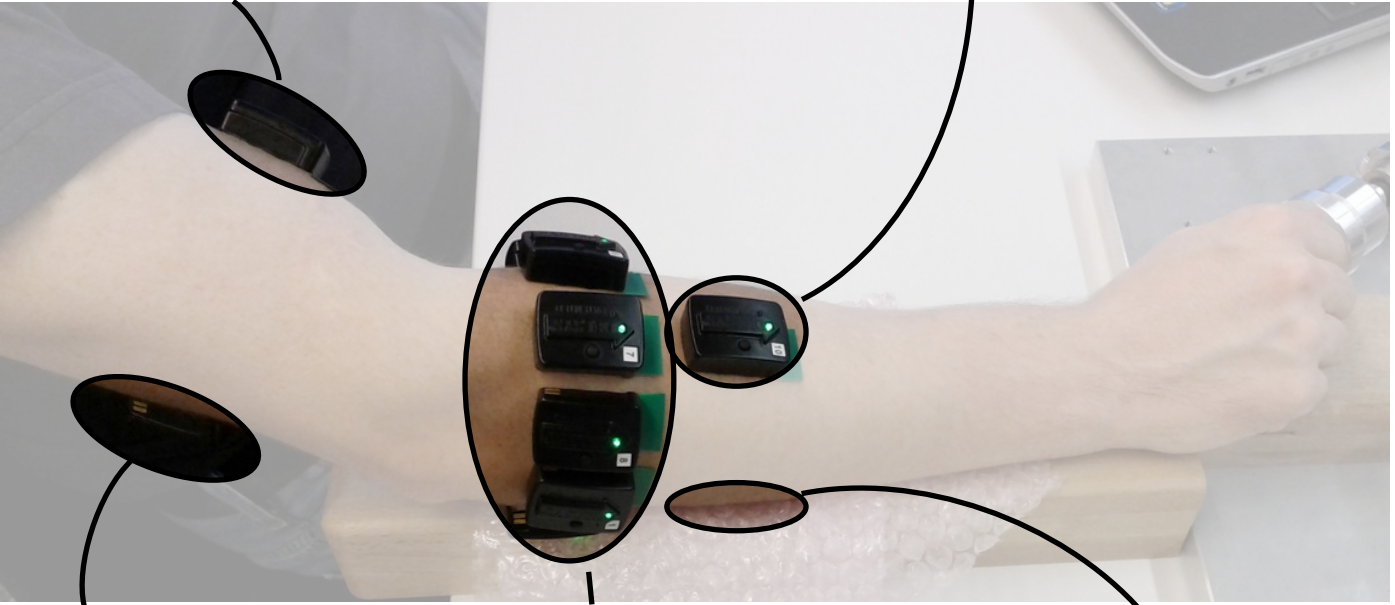
\includegraphics[width=4cm]{./img/eletrodos2.png}};
		\node [above=of eletrodos, yshift=-1.5em] {Eletrodos};
		\node [proc, fill=lcnorm!25, right=of eletrodos, yshift=4em] (EMG1) {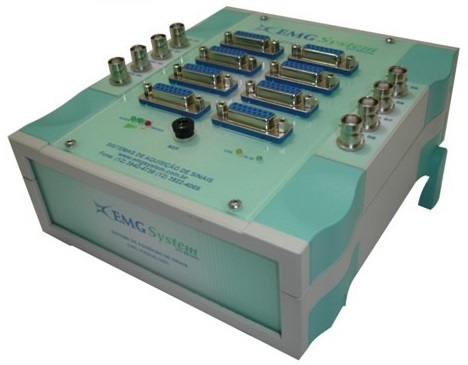
\includegraphics[width=3cm]{./flowcharts/EMG_830_C.jpg}};
		\node [proc, fill=lcnorm!25, right=of eletrodos, yshift=-4em] (EMG2) {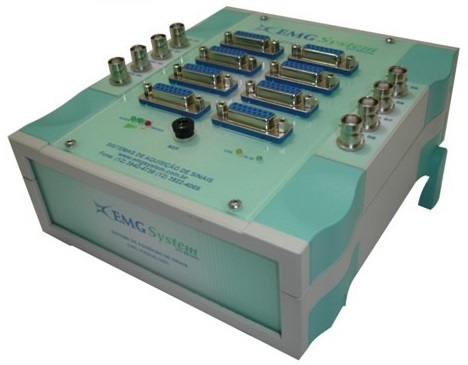
\includegraphics[width=3cm]{./flowcharts/EMG_830_C.jpg}};
		\node [above=of EMG2, yshift=-1.5em] {EMG 830C};
		\node [proc, fill=lccong!25, right=of EMG2, yshift=4em] (NI) {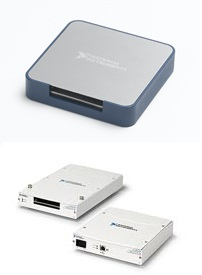
\includegraphics[width=3cm]{./flowcharts/ni_daq.jpg}};
		\node [above=of NI, yshift=-1.5em] {NI DAQ (SCB-68A e USB-6289)};
		\node [below=of NI] (labview) {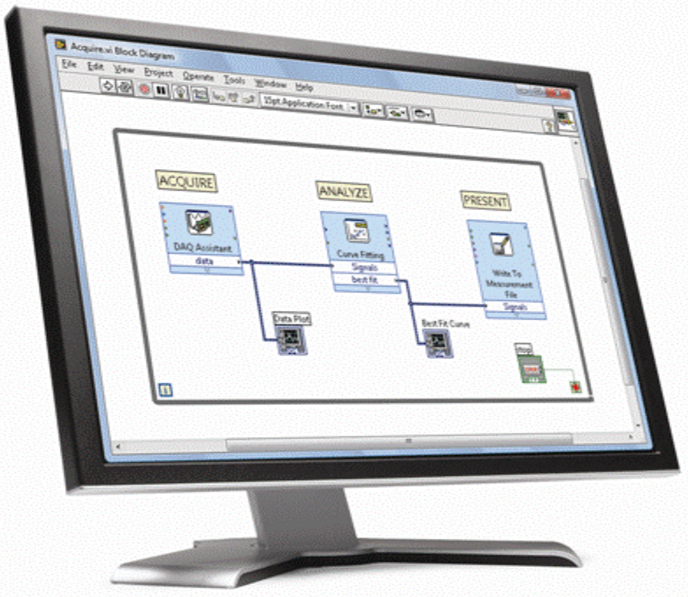
\includegraphics[width=3cm]{./img/labview.png}};
		\node [left=of labview, xshift=15em] {NI LabView};
		% -------------------------------------------------
%------------------------------------------------------------------------------
% Connections
%------------------------------------------------------------------------------
			\draw [->,black] (eletrodos) -- (EMG1);
			\path (eletrodos) to node [near start, yshift=2em, xshift=1em, align=center]{Canais \\ 1 a 8}(EMG1);
			\draw [->,black] (eletrodos) -- (EMG2);
			\path (eletrodos) to node [near start, yshift=-2em, xshift=1em, align=center]{Canais \\ 9 a 12}(EMG2);
			\draw [->,black] (EMG1) -- (NI);
			\draw [->,black] (EMG2) -- (NI);
			\draw [->,black] (NI) -- (labview);
		\end{tikzpicture}
		}
	\end{center}
	
\end{figure}
